\documentclass[twoside,10pt]{article}

\usepackage[labelsep=period,textfont=it]{caption}
\captionsetup[table]{name=TABLE}
\renewcommand{\thetable}{\Roman{table}}
\usepackage{lipsum,booktabs}
\usepackage[super]{natbib}
\usepackage{lipsum} % Package to generate dummy text throughout this template
\usepackage[sc]{mathpazo} % Use the Palatino font
\usepackage[T1]{fontenc} % Use 8-bit encoding that has 256 glyphs
\linespread{1.00} % Line spacing - Palatino needs more space between lines
\usepackage{microtype} % Slightly tweak font spacing for aesthetics
\usepackage{derivative}
\usepackage[hmarginratio=1:1,top=32mm,columnsep=20pt]{geometry} % Document margins
\usepackage{multicol} % Used for the two-column layout of the document
%\usepackage[hang, small,labelfont=bf,up,textfont=it,up]{caption} % Custom captions under/above floats in tables or figures
\usepackage{booktabs} % Horizontal rules in tables
\usepackage{float} % Required for tables and figures in the multi-column environment - they need to be placed in specific locations with the [H] (e.g. \begin{table}[H])
\usepackage{hyperref} % For hyperlinks in the PDF
\usepackage{multirow}
\usepackage{graphicx}
\usepackage{amsmath}
\usepackage{amsfonts}
\usepackage{amssymb}
\usepackage{lettrine} % The lettrine is the first enlarged letter at the beginning of the text
\usepackage{paralist} % Used for the compactitem environment which makes bullet points with less space between them
\usepackage{xcolor}
\usepackage{abstract} % Allows abstract customization
\renewcommand{\abstractnamefont}{\normalfont\bfseries} % Set the "Abstract" text to bold
\renewcommand{\abstracttextfont}{\normalfont\small\itshape} % Set the abstract itself to small italic text

\usepackage{titlesec} % Allows customization of titles
\renewcommand\thesection{\Roman{section}} % Roman numerals for the sections
\renewcommand\thesubsection{\Roman{subsection}} % Roman numerals for subsections
\titleformat{\section}[block]{\large\scshape\centering}{\thesection.}{1em}{} % Change the look of the section titles
\titleformat{\subsection}[block]{\large}{\thesubsection.}{1em}{} % Change the look of the section titles

\usepackage{fancyhdr} % Headers and footers
\pagestyle{fancy} % All pages have headers and footers
\fancyhead{} % Blank out the default header
\fancyfoot{} % Blank out the default footer
\fancyhead[C]{An Introduction to LabVIEW Fundamentals $\bullet$ November 7, 2021 } % Custom header text
\fancyfoot[RO,LE]{\thepage} % Custom footer text


%----------------------------------------------------------------------------------------
%	TITLE SECTION
%----------------------------------------------------------------------------------------

\title{\vspace{-15mm}\fontsize{15pt}{10pt}\selectfont\textbf{An Introduction to LabVIEW Fundamentals}} % Article title

\author{
	\small
	\textsc{Lauren Hernandez, Kathryn Wong}\\[1mm] % Your name
	\normalsize \textit{University of Houston}\\ % Your institution
	\normalsize \textit{Physics 3313: Advanced Laboratory I}\\ % Your Course
%	\normalsize \href{mailto:john@smith.com}{john@smith.com} % Your email address
	\vspace{-10mm}
}
\date{}

%----------------------------------------------------------------------------------------

\begin{document}
	
	\maketitle % Insert title
	
	\thispagestyle{fancy} % All pages have headers and footers
	
	%----------------------------------------------------------------------------------------
	%	ABSTRACT
	%----------------------------------------------------------------------------------------
	
	\begin{abstract}
		
	\noindent Fundamental knowledge of LabVIEW was gained in this experiment through setting up a boolean program, testing and calibrating equipment, working with voltage data aquisition, and processing signals created by voice and tuning forks. The resonant frequency of the unlabeled tuning fork was $325 \text{Hz}$. 

		
	\end{abstract}
	
	%----------------------------------------------------------------------------------------
	%	INTRODUCTION
	%----------------------------------------------------------------------------------------
	
	\begin{multicols}{2} % Two-column layout throughout the main article text
		
		\section{Introduction} 
		
			\lettrine[nindent=0em,lines=2]{I}n many circumstances, the tasks of a researcher, working-professional or student, may include building complex systems or processing large amounts of information. When these circumstances arise, complicated tasks have the potential to turn into one-step executions with the aid of computer programming. LABVIEW is a graphical programming language with various applications, including data aquisition, test automation, embedded system design, industrial/instrument control, and analysis and signal processing $^1$. 
			
			\indent The goal of this experiment is to gain experience with LabVIEW for assisted data aquisition, instrument testing, and instrument control to ultimately determine the resonant frequency of a tuning fork. 
			
	%	EXPERIMENTAL PROCEDURE
	%----------------------------------------------------------------------------------------
		
		\section{Experimental Procedure}
		
		\subsection*{Equipment}
		The equipment we used for this experiment were LabVIEW 2012 software, DAQ Series X Manual, Lenovo Windows Computer, Acer Computer Screen Monitor, EXTECH Instruments True RMS Multimeter EX430A, Nady Audio SMPS - 1X adapter YL1800350, NI CB 68-LP Connection Block, phantom power supply 1971504645, Behringer C-2 condenser microphone J1417034263, a rubber mallet, and three tuning forks of frequency 435 Hz, 256 Hz and one of an unknown frequency.
		
		\subsection*{Part One: Simple Boolean Program}
		We opened LabVIEW and created a blank VI. In the Front Panel window, we put two switches naming them "Premise A" and "Premise B", and put four indicators, naming them "A", "B", "A and B" and "A or B", shown below in Figure 1. 
		
		\setlength{\textfloatsep}{10pt plus 1.0pt minus 2.0pt}
			\begin{figure}[H]
			\centering
			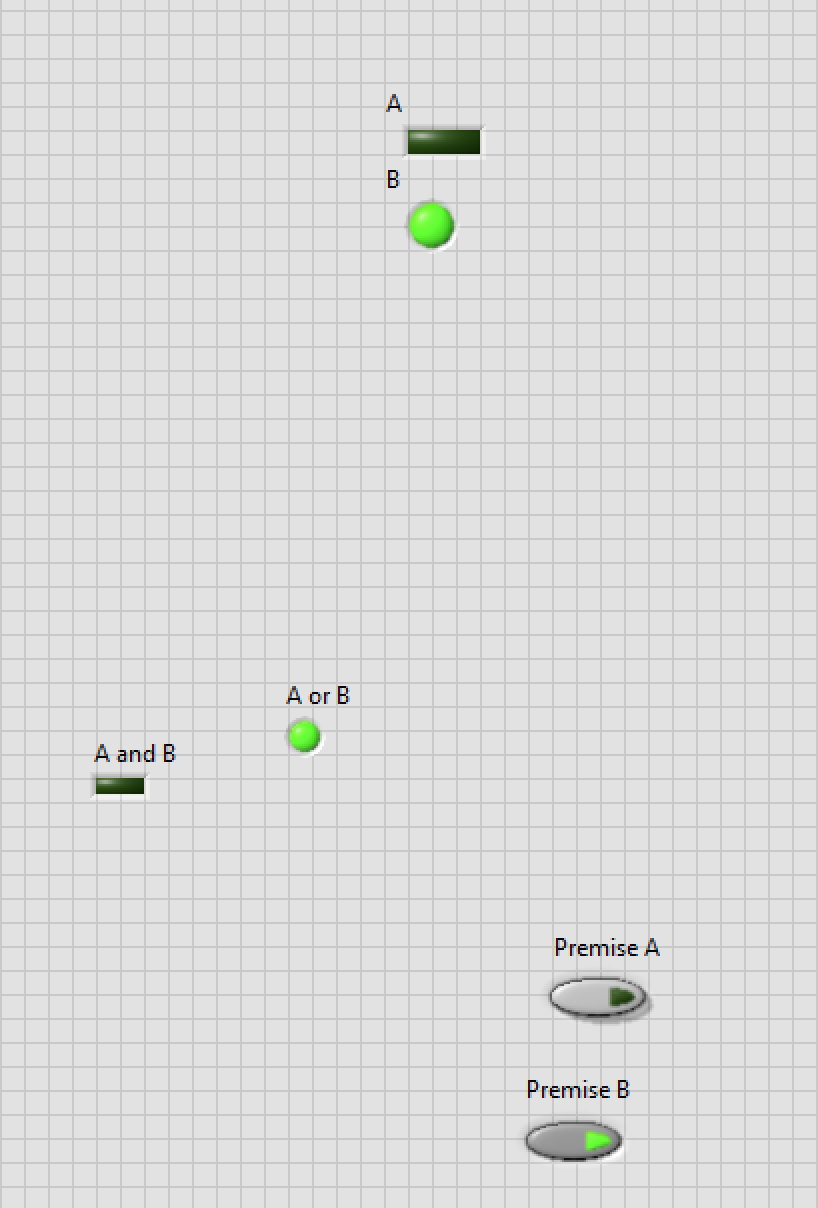
\includegraphics[width=46mm]{boolean front panel group 4 1.png}
			\caption{Two switches and four indicators located in the Front Panel window, used to set up a simple boolean program. }
		\end{figure}
		
		
		We went to the Block Diagram window, arranged the switches vertically downward, and wired "Premise A" to "A" and "Premise B" to "B".We then returned to the Front Panel, changed the truth value of a random switch, and then ran the program by clicking "Run". We then clicked "Run Continuously", followed by "Abort Execution". We returned to the Block Diagram window and clicked "Highlight Execution" and then ran the program again. We right clicked in an empty space in the Block Diagram window, pulled up the Functions Palette, placed a boolean "And" to the left of the "A and B" indicator, and placed an "Or" to the left of the "A or B" indicator. We wired "Premise A" and "Premise B" to the "And" conditional, ran the program, received an error, and then made connections to the "Or" conditional. Then, we deselected "Highlight Execution", went to the Front Panel window and ran the program continuously. We returned to the Functions Palette, selected a While Loop and placed all of our code inside of the While Loop. We added a control to the Stop Control terminal on the loop, and placed a "Wait Function" inside the loop in the Block Diagram window. We placed a numeric constant of 100 inside the loop, wiring it to the left input of terminal of the "Wait Function". Then, we returned to the Front Panel window and clicked run, as shown below in Figure 2.
		
		\vspace{-10pt}
		
			\begin{figure}[H]
			\centering
			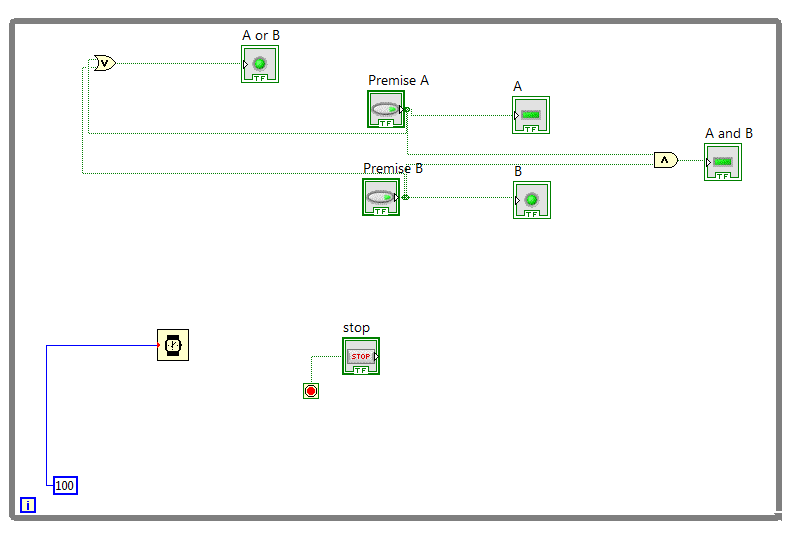
\includegraphics[width=\linewidth]{boolean block diagram group 4.png}
			\caption{A simple boolean program displayed in the Block Diagram window of LabVIEW.}
		\end{figure}
		
		
		\subsection*{Part  Two: The Measurement and Automation Explorer (NI MAX)}
		
		We checked the connection between the Connection Block and the DAQ card on the computer, opened the NI-MAX icon on the desktop, clicked "Devices and Interfaces" and selected "NI PCI-6014". We right clicked the device name and selected "Device Pinouts", shown below in Figure 3.
		
			\begin{figure}[H]
			\centering
			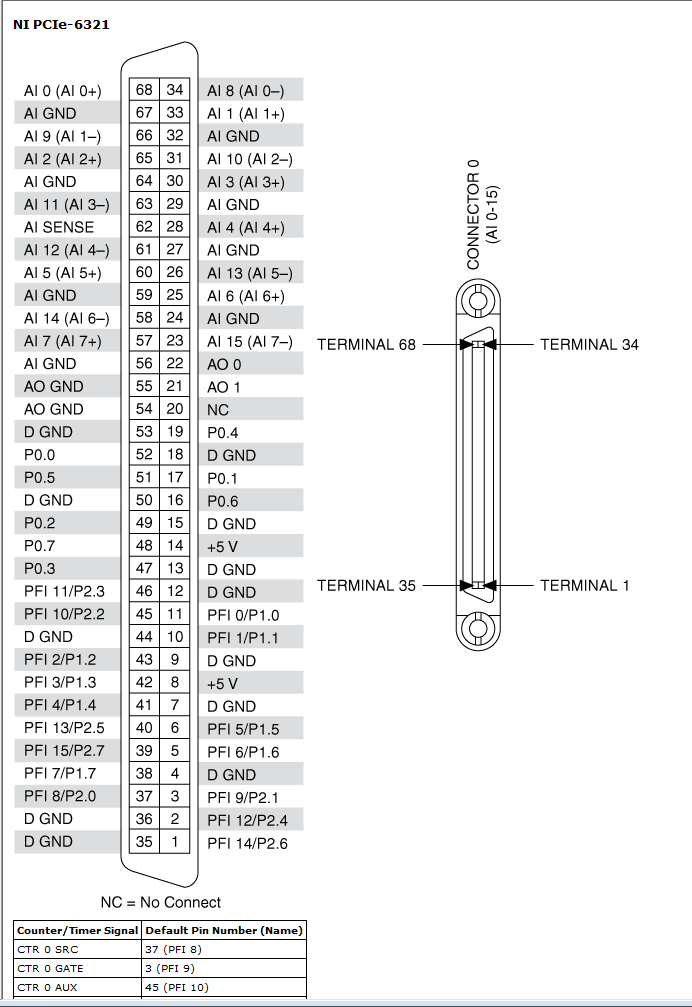
\includegraphics[width=65mm]{group 4 part 2 device pin outs.png}
			\caption{Device pinout diagram for NI PCI-6014 device.}
		\end{figure}
		
		We clicked the "Self Test" button, checked to make sure all of the terminals on the Connection Block were open, and then clicked "Self-Calibrate". We connected a DC voltage source of 6 volts in Non-Referenced Single Ended mode (NRSE) to the input channels on the Connection Block. We selected input 68, 62, and 56, which correspond to AChannel0, AISENSE, and AIGround. We clicked "Test Panels", clicked the channel connected to the voltage source, set the Mode to "Continuous", set the configuration to NRSE, and clicked start. We then recorded the voltage when measured by a multimeter. Then, we switched from AChannel0 to DAC0OUT, and measured the voltage with a multimeter.  
		
		
		\subsection*{Part Three: Simple Voltage Measurement Program}
		
		We created a new VI, and added a DAQ Assistant to the Block Diagram window. We selected "Aquire Signals", "Analog Input", "Voltage", "ai0", and then "Finish". We set the Signal Input Range to 0-10, set the Terminal Configuration to NRSE, Aquisition Mode to "N Samples", and clicked "OK". We created controls for "Number of Samples" and "Rate", and then created a "Graph Indicator" for the "data" terminal output. In the Block Diagram window, we created a blank "Array Constant" and put a "Double Numeric Constant" inside of it, and changed it to an indicator. We wired the DAQ Assistant data output to the array, and expanded the indicator for the array to show multiple output values. Then, we ran the program. We returned to the Block Diagram window and added "Array Max \& Min", "Add Array Elements", and "Divide" functions. We wired the DAQ Assistant's data output terminal to "Array Max \& Min" and "Add Array Elements", and wired "Add Array Elements" and "Numher of Samples" to the "Divide" function. We then made indicators for Max, Min and Divide and ran the program. In the Block Diagram window, we added a "Write to Spreadsheet File" function, wired controls to file path and format terminals, and wired a constant to "transpose". We entered a filepath for the data and wired the array to the "Write Spreadsheet" input and ran the program. Then, we highlighted all of the functions and VI's in the Block Diagram windowNd created a SubVI, and saved it. 
		
		
		
		\subsection*{Part Four: Introduction to Signal Processing}
		
		We connected a microphone to a phantom microphone and wired the phantom power supply to an analog channel on the DAQ Connection Block in NRSE mode. We left the connections at the Connection Block set up as we had it in part three of the experiment. Then, we switched the phantom power unit on. We created a new VI, and put a DAQ Assistant VI in the Block Diagram window. We wired controls to the DAQ Assistant for "Stop", "Number of Samples", and "Sample Rate". We then wired a "Waveform Graph" to the "data" output. We varied the value for "Number of Samples" and "Rate" and noticed the difference in output plots. Then, we placed a "Convert" from the "Dynamic" function into the Block Diagram window and set it to output a "Single Waveform", by wiring the signal output to the conversion function. We put an FFT Power Spectrum VI in the Block Diagram window, and connected the output of the conversion function to the "Time Signal" on the FFT power spectrum. We put 'Unbundle By Name" into the Block Diagram window and wired it to the FFT Power Spectrum. Then we wired the output, "Magnitude" array, to a second waveform graph and created a second graph on the Front Panel window; then we ran the program. Then we used the two labeled tuning forks and our voices while saying the word "Hello" to understand the relationship between the number of samples, sample rate, FFT frequency and the time over which the data was collected. Then, we used this information to interpret the FFT plot of the unknown tuning fork. 
		
		
	%----------------------------------------------------------------------------------------
	%	RESULTS, ANALYSIS AND DISCUSSION
	%----------------------------------------------------------------------------------------
		\section{Results, Analysis, Discussion}
		
		
		\subsection*{Part One: Simple Boolean Program}
		
			The resulting boolean program was set up in both the Front Panel window and in the Block Diagram window, as seen in Figures 1 and 2 in the experimental procedure section. When the switches are green, they are in "On" mode, and when the switches are not green, they are in "Off" mode. We set up the program to where one of each switch or indicator pairs was on and one was off. We set "A" to be "Off", and "B" to be "On"; we set "A and B" to be "Off", and "A or B" to be "On"; and we set "Premise A" to be "Off" and "Premise B" to be "On". The program ran seamlessly, so long as "Premise A" and "Premise B" were connected to at least one switch. We connected the premise indicators, each to three switches, so that there could be various outcomes depending on which switch was "On" and which switch was "Off".

				
		\subsection*{Part  Two: The Measurement and Automation Explorer (NI MAX)}
		
			The voltage source was labeled as having a  6V power supply, and the test pannel produced a voltage reading of $6.00 \text{V} \pm 1\text{V}$ for connections to both A1GND and A0GND. The multimeter produced a steady reading of $6.00 \text{V} \pm 1 \text{V}$ for connections to both A1GND and A0GND. The test pannel reading and multimeter reading for connections to A1GND and A0GND are shown below in Table 1 and Table 2. 
		
			\begin{table}[H]
			\centering
			\caption{Test panel and multimeter reading of a 6V voltage source, using a Connection Block's A1GND terminal. }
			\begin{tabular}{l c c rrrrrrr}
				\toprule				
				A1GND & Test Pannel & Multimeter  \\ [1ex]
				\midrule
				&	6.01 V & 6.01 V  \\ [1.5ex]
				&	6.00 V & 6.01 V  \\ [1.5ex]
				&	6.02 V & 6.01 V \\ [1.5ex]
				\bottomrule
			\end{tabular}
		\end{table}
	
		\begin{table}[H]
		\centering
		\caption{Test panel and multimeter reading of a 6V voltage source, using a Connection Block's A0GND terminal.}
		\begin{tabular}{l c c rrrrrrr}
			\toprule				
			A0GND & Test Pannel & Multimeter  \\ [1ex]
			\midrule
			&	6.00 V & 6.01 V  \\ [1.5ex]
			&	6.01 V & 6.01 V  \\ [1.5ex]
			&	6.00 V & 6.01 V \\ [1.5ex]
			\bottomrule
		\end{tabular}
	\end{table}
		
		The output waveforms of the voltage (amplitude) vs. samples taken while using terminal A1GND and A0GND are shown below in Figure 4 and Figure 5.
		
		\begin{figure}[H]
			\centering
			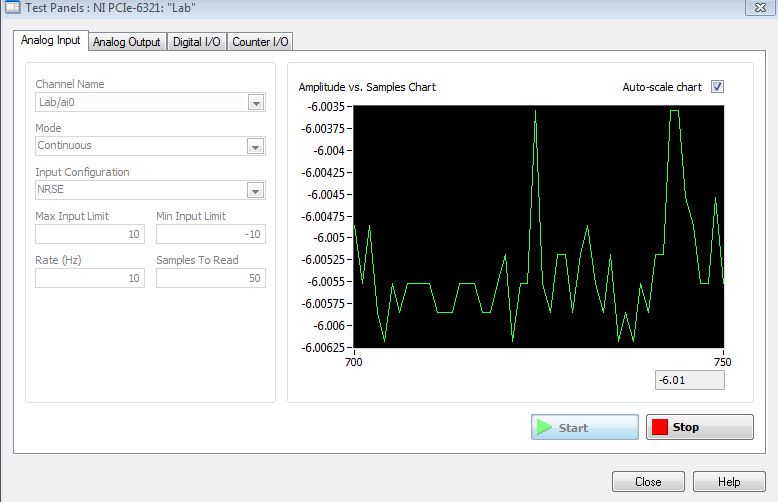
\includegraphics[width=\linewidth]{group 4 voltage waveform.png}
			\caption{Voltage (amplitude) vs. Samples of a 6V power source, using a Connection Block's A1GND terminal. }
		\end{figure}
		
		\begin{figure}[H]
			\centering
			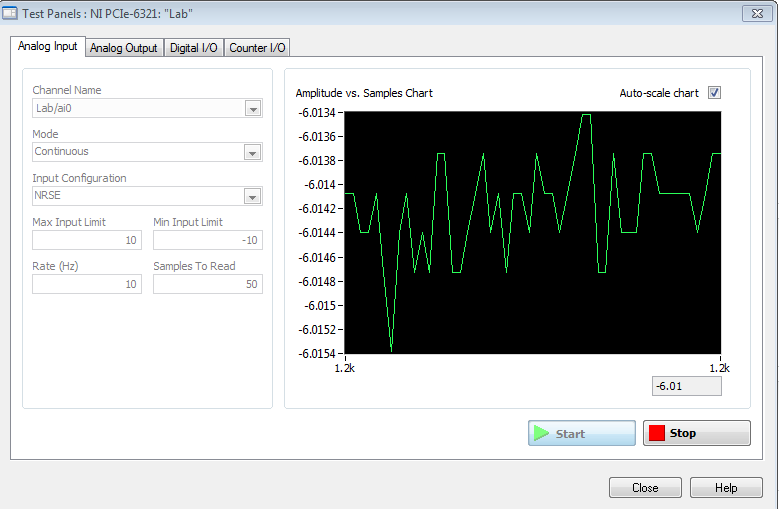
\includegraphics[width=\linewidth]{group 4 voltage output for aoground.png}
			\caption{Voltage (amplitude) vs. Samples of a 6V power source, using a Connection Block's A0GND terminal. }
		\end{figure}
	
		\indent The sample rate was an important variable in when we were gathering data for the voltage reading, because the higher the rate was, the more data we were collecting per second. This was useful, becuase the more data we had, the more accurately the voltage over time curve represented the actual voltage of the power supply. 

		There were no complications with this part of the experiment. The test pannel and multimeter readings both confirmed the value of the voltage source. The success of this part of the experiment could be due to the fact that we made sure the connections we placed between the voltage source, the terminals in the connection block, the computer, and mulitmeter were all secure and in-tact throughout the experiment. Additionally, we tested the functions on the multimeter prior to using it, to make sure that it was fully functional for the experiment. 
		
		\subsection*{Part Three: Simple Voltage Measurement Program}
		
		After we set up the program, the average output reading of the 6V power source was 6.01069 V. The output waveform of voltage over time is shown below in Figure 6. 
		
			\begin{figure}[H]
			\centering
			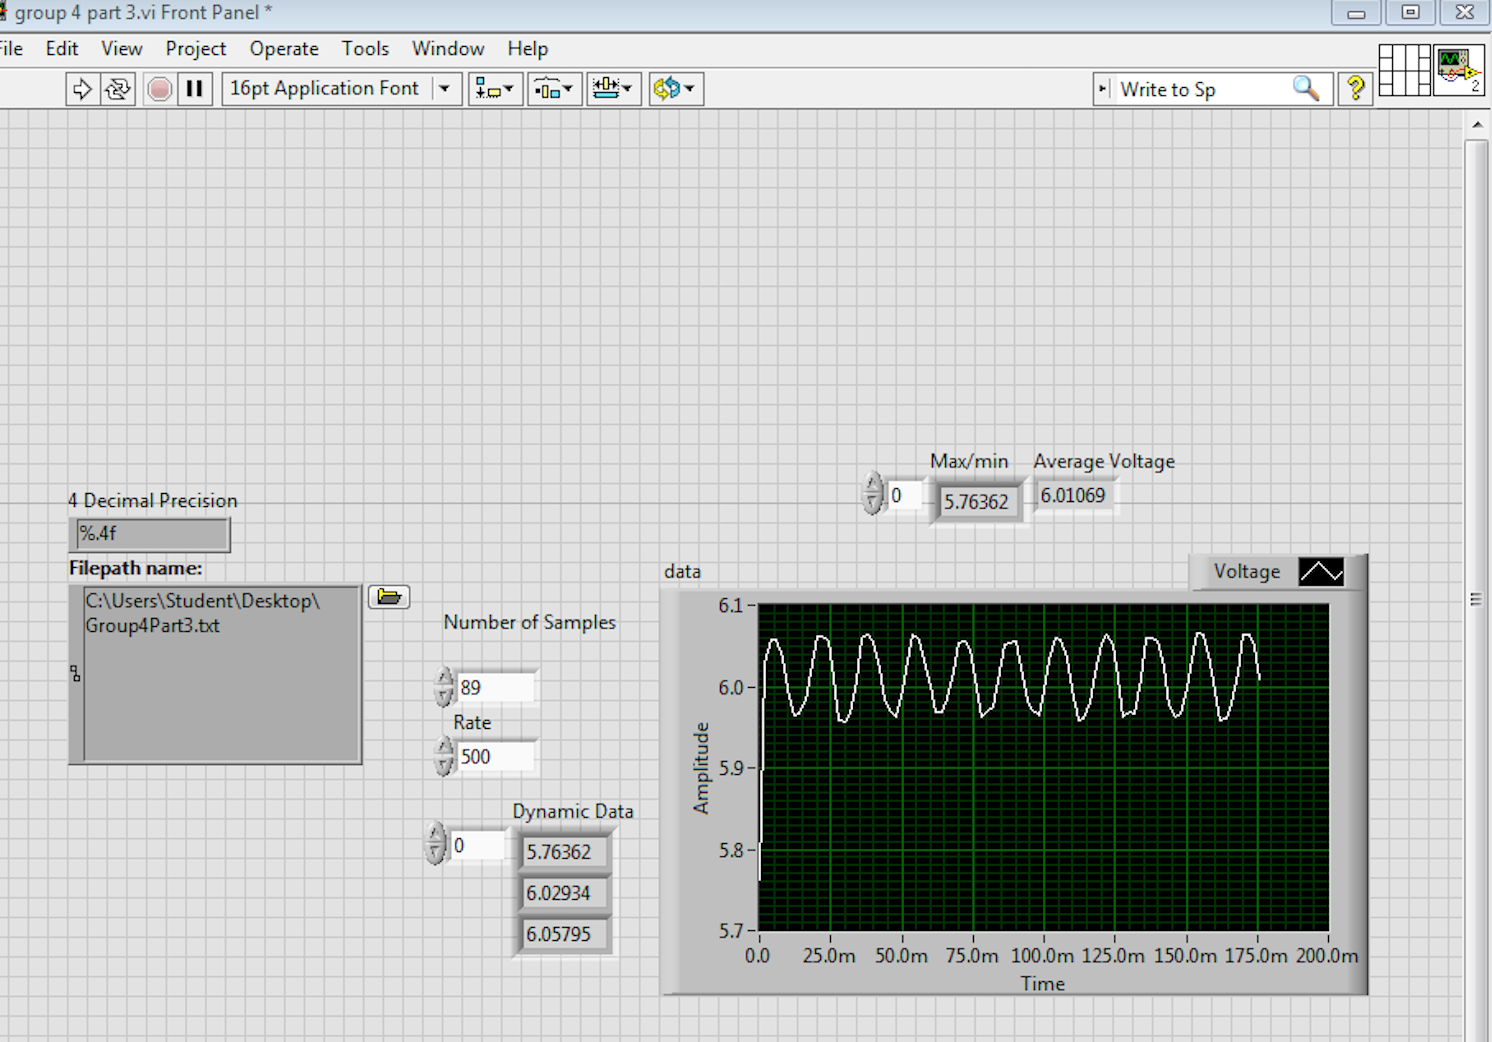
\includegraphics[width=\linewidth]{1.png}
			\caption{Voltage measurement function,voltage (amplitude) vs time, shown in the Front Pannel window using a 6V power source. The desired filepath chosen is visible from the window.}
		\end{figure}
		
		Shown below in Figure 7 is the Block Diagram window after we finished setting up the program and checked it for errors.
		
			\begin{figure}[H]
			\centering
			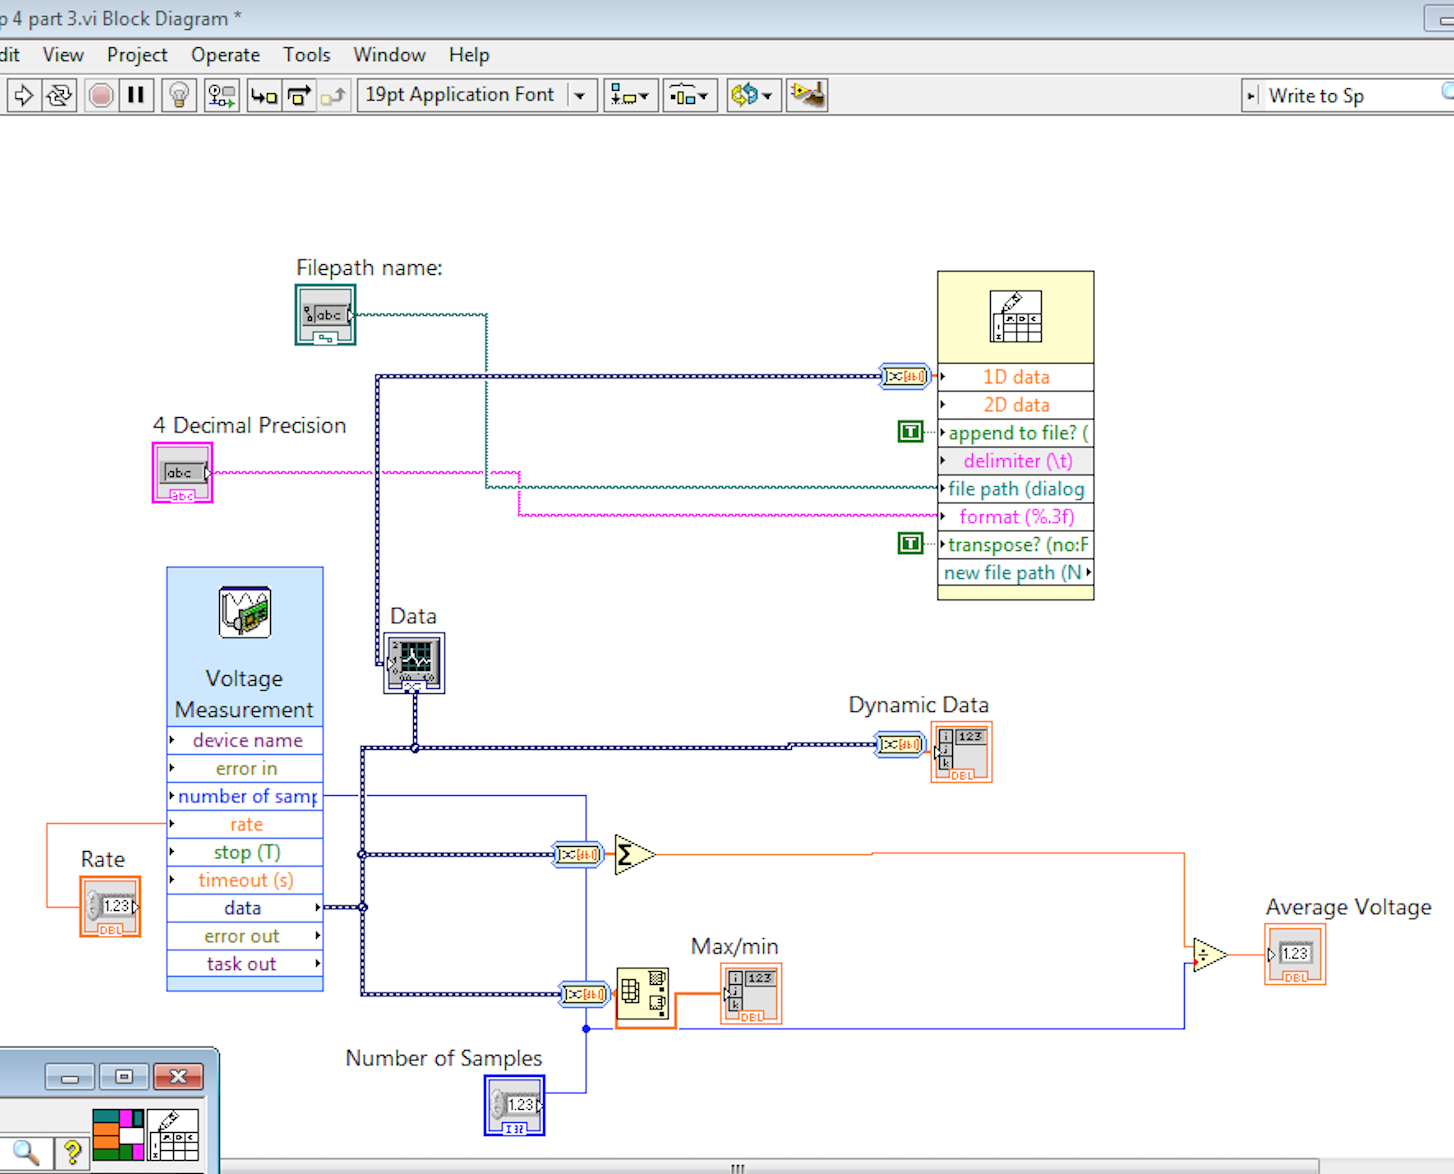
\includegraphics[width=\linewidth]{2.png}
			\caption{Voltage measurement program set up in the Block Diagram window using a 6V power source.}
		\end{figure}
	
		Shown below in Figure 8 is the "Write to Spreadsheet" VI in a sub- Front Panel window. In this widow, we specified the filepath that we wanted to use for data collection, we specified a 4 digit decimal precision, and we chose to not transpose our data.
	
		\begin{figure}[H]
		\centering
		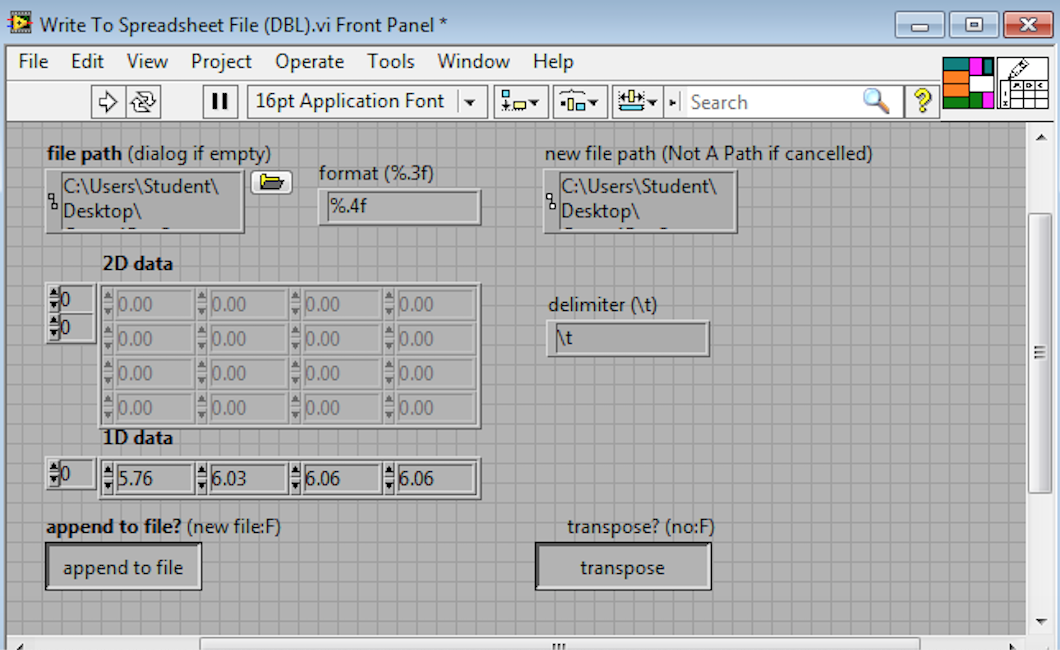
\includegraphics[width=\linewidth]{3.png}
		\caption{Shown is the "Write to Apreadsheet" command that was set up in the Block Diagram window, with sample data displayed to a 4-point decimal precision, and the chosen filepath displayed.}
	\end{figure}
		
		We had no unsolvable errors with this part of the experiment. Kathryn and I both have experience with programming, and we set up the program as instructed and the program ran without bugs. We left the Command Block set up securely, as it was in the prior parts of the experiment, and this could have contributed to the success of part three of the experiment. 
		
		\subsection*{Part Four: Introduction to Signal Processing}

		When striking each tuning fork with the rubber mallet, we output two plots. One voltage plot, which is represented as amplitude vs time, and a plot of the Fast Fourier Transform of the voltage plot, represented as intensity vs frequency. The voltage plot was produced by turning sound waves into a volatage wave, and the peaks and pits in the voltage plot represent the rise and fall of how the tuning fork sounds when struck - it sounds like an oscillating ringing, with waves of "loudness" followed by a wave of "quietness". The Fast Fourier Transform of the voltage wave showed us all of the different frequencies that compiled, and superimposed to create the overall sound given off by the respective tuning fork. Each tuning fork's total frequency was made by the summation of several frequencies and those several frequencies are shown in the Fast Fourier Transform plot, showing to what ratio, or quantity, did each coomponent frequency contribute to the overall sound of the tuning fork.
		
		Shown below in Figure 9 are the output voltage and FFT plots of a 256 Hz tuning fork when struck with a rubber mallet.
		
		\begin{figure}[H]
		\centering
		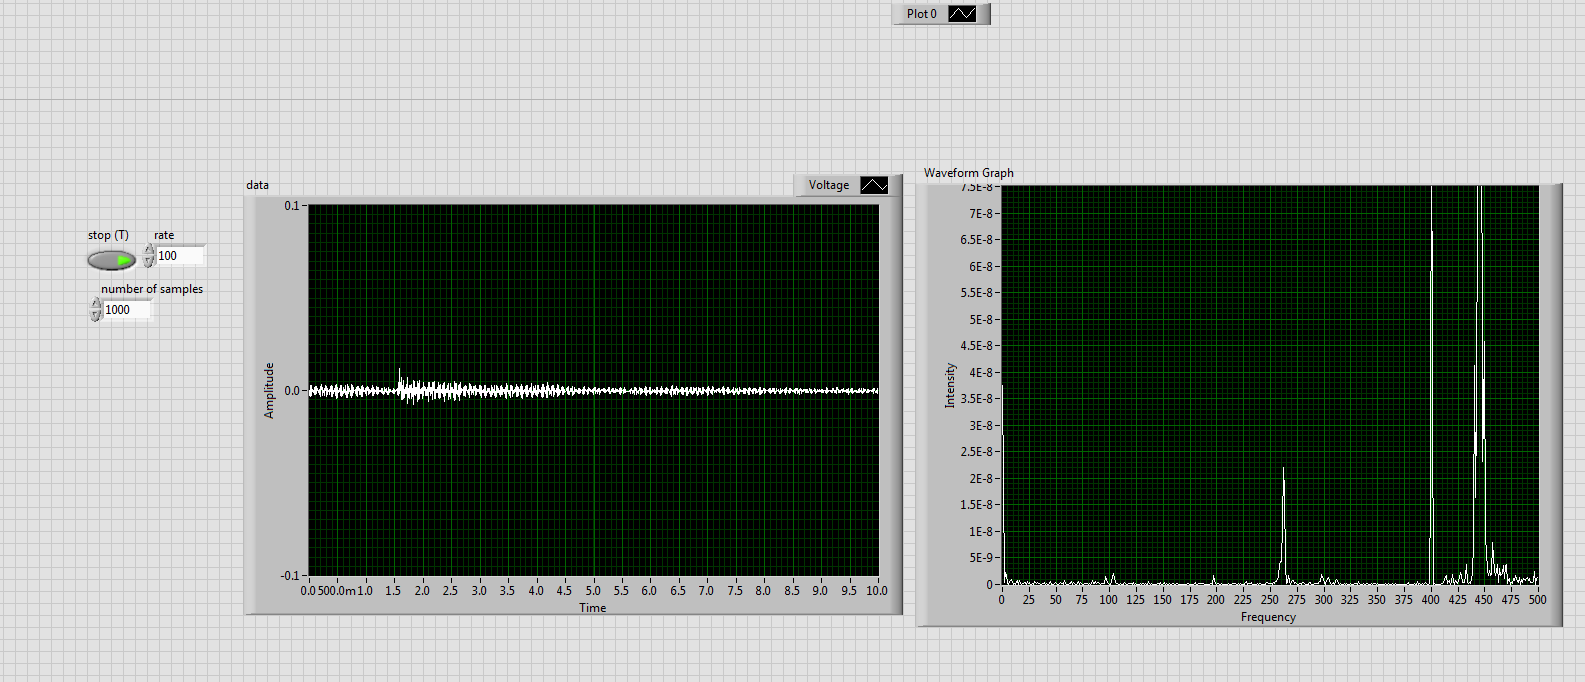
\includegraphics[width=\linewidth]{group4_256_waveform.png}
		\caption{Shown above on the left is the voltage waveform, and on the right is the FFT of the voltage waveform; both curves represent a 256 Hz tuning fork after it was struck with a rubber mallet.}
		\end{figure}
	
			Shown below in Figure 10 are the output voltage and FFT plots of a 435 Hz tuning fork when struck with a rubber mallet.
	
	
		\begin{figure}[H]
		\centering
		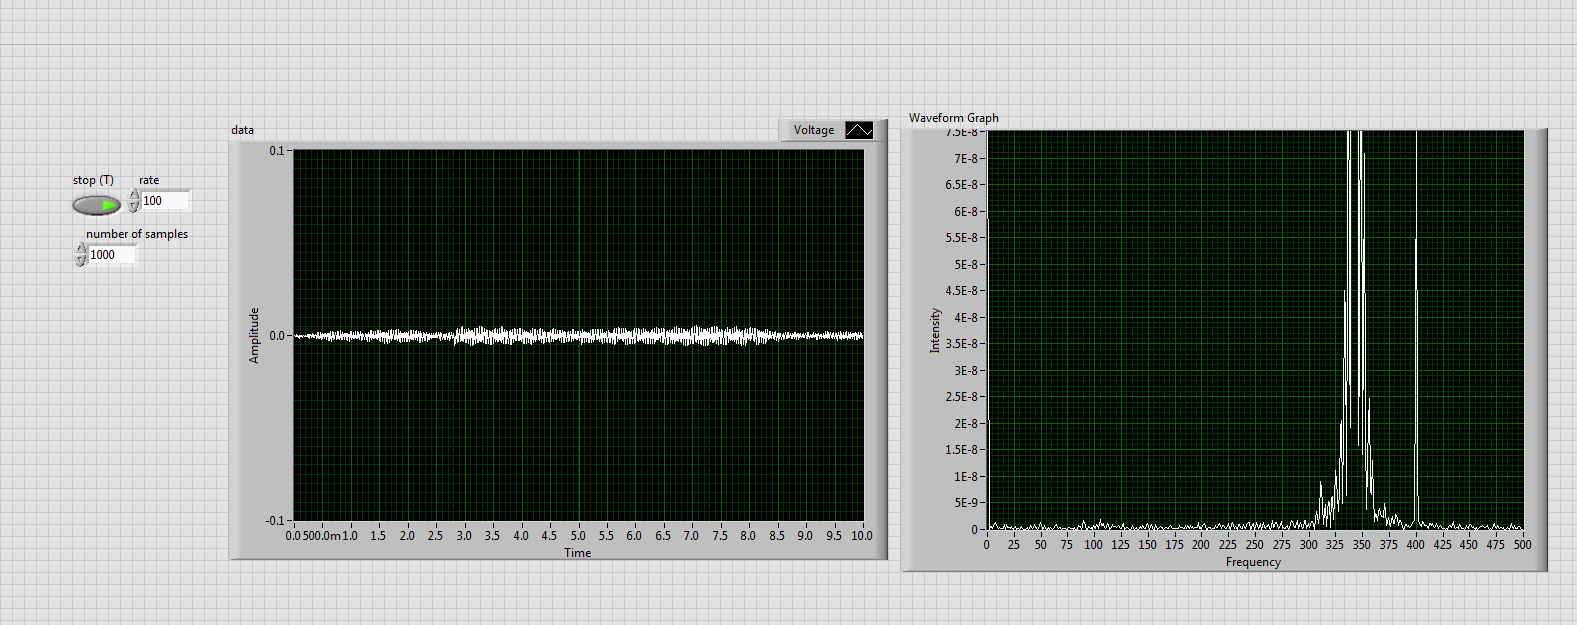
\includegraphics[width=\linewidth]{group4_435_waveform.png}
		\caption{Shown above on the left is the voltage waveform, and on the right is the FFT of the voltage waveform; both curves represent a 435 Hz tuning fork after it was struck with a rubber mallet.}
		\end{figure}
	
				Shown below in Figure 11 are the output voltage and FFT plots of a  tuning fork of unknown frequency when struck with a rubber mallet.
	
		\begin{figure}[H]
		\centering
		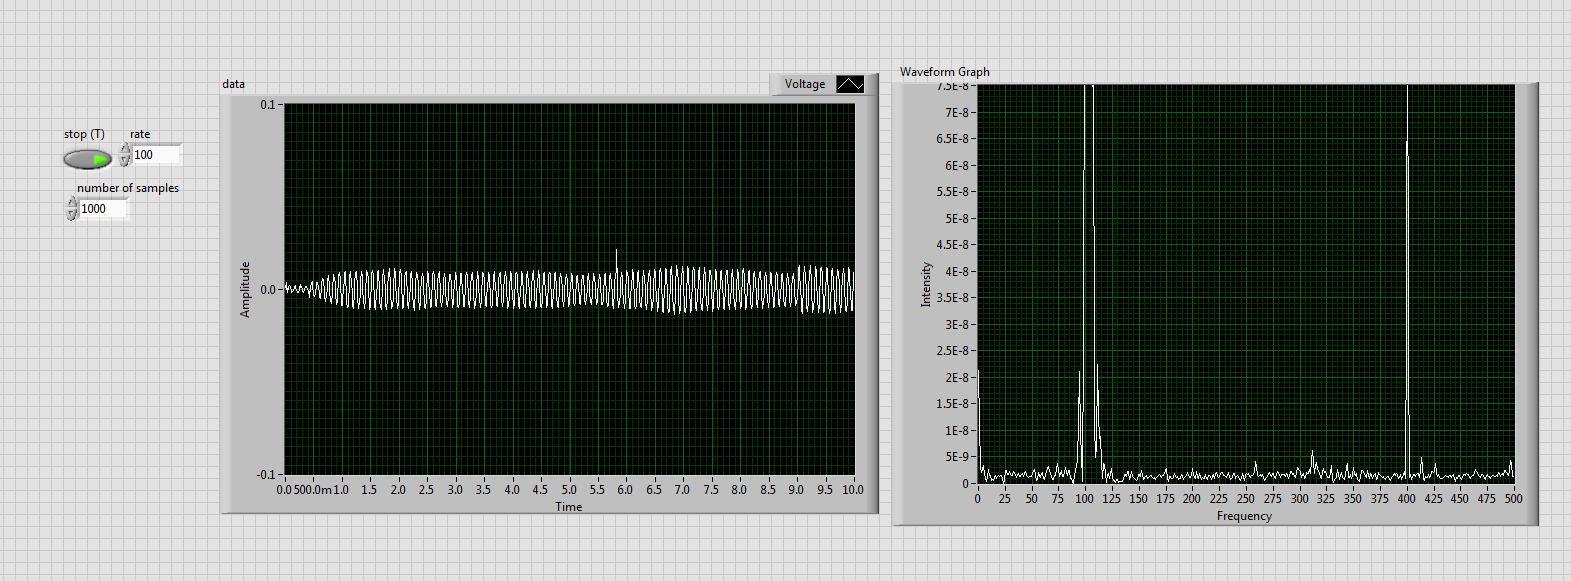
\includegraphics[width=\linewidth]{group4_unknown_waveform.png}
		\caption{Shown above on the left is the voltage waveform, and on the right is the FFT of the voltage waveform; both curves represent a tuning fork of unknown frequency after it was struck with a rubber mallet.}
		\end{figure}
	
		Further, in each voltage plot, the amplitude represents the amount of voltage recorded over time. In each FFT plot of the voltage, the intensity represents the magnitude to which each contributing frequency is present in the overall total frequency of the tuning fork, and the freqency lists range of frequencies present. The frequency of the unknown tuning fork was determined to be 325Hz.
	%----------------------------------------------------------------------------------------
	%	CONCLUSIONS
	%----------------------------------------------------------------------------------------
		\section{Conclusion}
		In conclusion, LabVIEW is a program that utilizes programming in a digaram format to process information, and is quite easy to use. The simple boolean program was straightforward and the programming involved helped in understanding how to navigate through LabVIEW. Part two and three of the experiment proved the degree of accuracy to which LabVIEW can test various equipment. Lastly, part four of the experiment gave the results of the frequency of an unknown tuning fork, which was 325 Hz. 

		
		
	%	REFERENCE LIST
	%----------------------------------------------------------------------------------------
		\begin{thebibliography}{99} % Bibliography - this is intentionally simple in this template
			\raggedright
			\bibliography{mybib}
	\begin{small}
	\bibitem[1]{2001}
	Wikimedia Foundation. (2021, November 7). LabVIEW. Wikipedia. Retrieved November 7, 2021, from \textcolor{blue}{https://en.wikipedia.org/wiki/LabVIEW}. 

	\bibitem[2]{2002}
	DAQ NI 6013/6014 User Manual, National Instruments,available in Phys 3313 laboratory and at \textcolor{blue}{https://kur.web.psi.ch/sans1/manuals
	/NI\%206013\%20and\%206014\%20User\%20Man
	ual.pdf}, accessed November 7, 2021.
	
	\bibitem[3]{2003}	
	\textit{DAQ E Series User Manual}, National Instruments \textcolor{blue}{http://www.ni.com/pdf/manuals/370503k.pdf}, accessed November 7, 2021.

	\bibitem[4]{2004}
	Ulinski, A. \& Forrest, R. L., "Lab Manual for Advanced Laboratory I", Physics 3313, \textit{A Crash Course in LabVIEW Fundamentals}, pages 1 - 8, (The University of Houston, 2021).
	
\end{small}

	
\end{thebibliography}
		
	%----------------------------------------------------------------------------------------
		
	\end{multicols}
	
\end{document}